\documentclass[10pt]{beamer}
\usepackage{ceai-beamer}
\usepackage{ragged2e}
\usepackage{amsmath,amssymb}
\usepackage{graphicx}
\usepackage{subcaption}
\usepackage{bm}
\usepackage{hyperref}

\graphicspath{{../figs/}{./figs/}}

\title[Topic 5 Part 1]{CE 488/5588: Applied Machine Learning\\\large Topic 5: Introduction to Neural Networks (Part 1)}
\author{}
\date{}

\begin{document}

\begin{frame}[plain]
  \titlepage
\end{frame}

\begin{frame}{Outline}
  \justifying
  \tableofcontents
\end{frame}

\section{Introduction}

\begin{frame}{Why Neural Networks?}
  \justifying
  Artificial neural networks (ANNs) provide a flexible supervised learning model that can capture complex, nonlinear relationships.
  They were inspired by biological neural systems but are expressed as compact mathematical models.

  \vspace{0.5em}
  \footnotesize
  Historical context: \href{https://news.cornell.edu/stories/2019/09/professors-perceptron-paved-way-ai-60-years-too-soon}{news.cornell.edu/...}
\end{frame}

\begin{frame}{Historical Milestones}
  \justifying
  \begin{itemize}
    \item 1958: Frank Rosenblatt builds the first perceptron machine.
    \item 2012: CNNs achieve a breakthrough on ImageNet (AlexNet).
    \item Modern deep learning builds on multilayer perceptrons and large-scale optimization.
  \end{itemize}
  \vspace{0.5em}
  \footnotesize
  Sources: \href{https://www.ling.upenn.edu/courses/cogs501/Rosenblatt1958.pdf}{ling.upenn.edu/...},
  \href{https://proceedings.neurips.cc/paper/4824-imagenet-classification-with-deep-convolutional-neural-networks.pdf}{proceedings.neurips.cc/...}
\end{frame}

\begin{frame}{Learning Objectives}
  \justifying
  After completing this topic, you should be able to:
  \begin{itemize}
    \item Write a single-neuron (perceptron) model in vector form and interpret weights and bias.
    \item Explain how activation functions affect optimization (saturation, vanishing gradients, dying ReLUs).
    \item Choose appropriate output-layer/activation and loss pairs for common tasks.
    \item Explain why a single linear decision boundary cannot solve XOR.
    \item Describe, at a high level, how backpropagation applies the chain rule.
  \end{itemize}
\end{frame}

\begin{frame}{Terminology}
  \justifying
  \begin{conceptbox}{Key Terms}
    \begin{itemize}
      \item \textbf{Perceptron (classic):} linear classifier with a hard threshold activation.
      \item \textbf{Logistic regression (single neuron):} sigmoid output with probabilistic interpretation, trained via cross-entropy.
      \item \textbf{MLP:} feedforward network with one or more hidden layers trained via gradient-based methods.
    \end{itemize}
  \end{conceptbox}
\end{frame}

\section{Neuron Cell and Perceptron}

\begin{frame}{Biological Inspiration}
  \justifying
  \begin{figure}[ht]
    \centering
    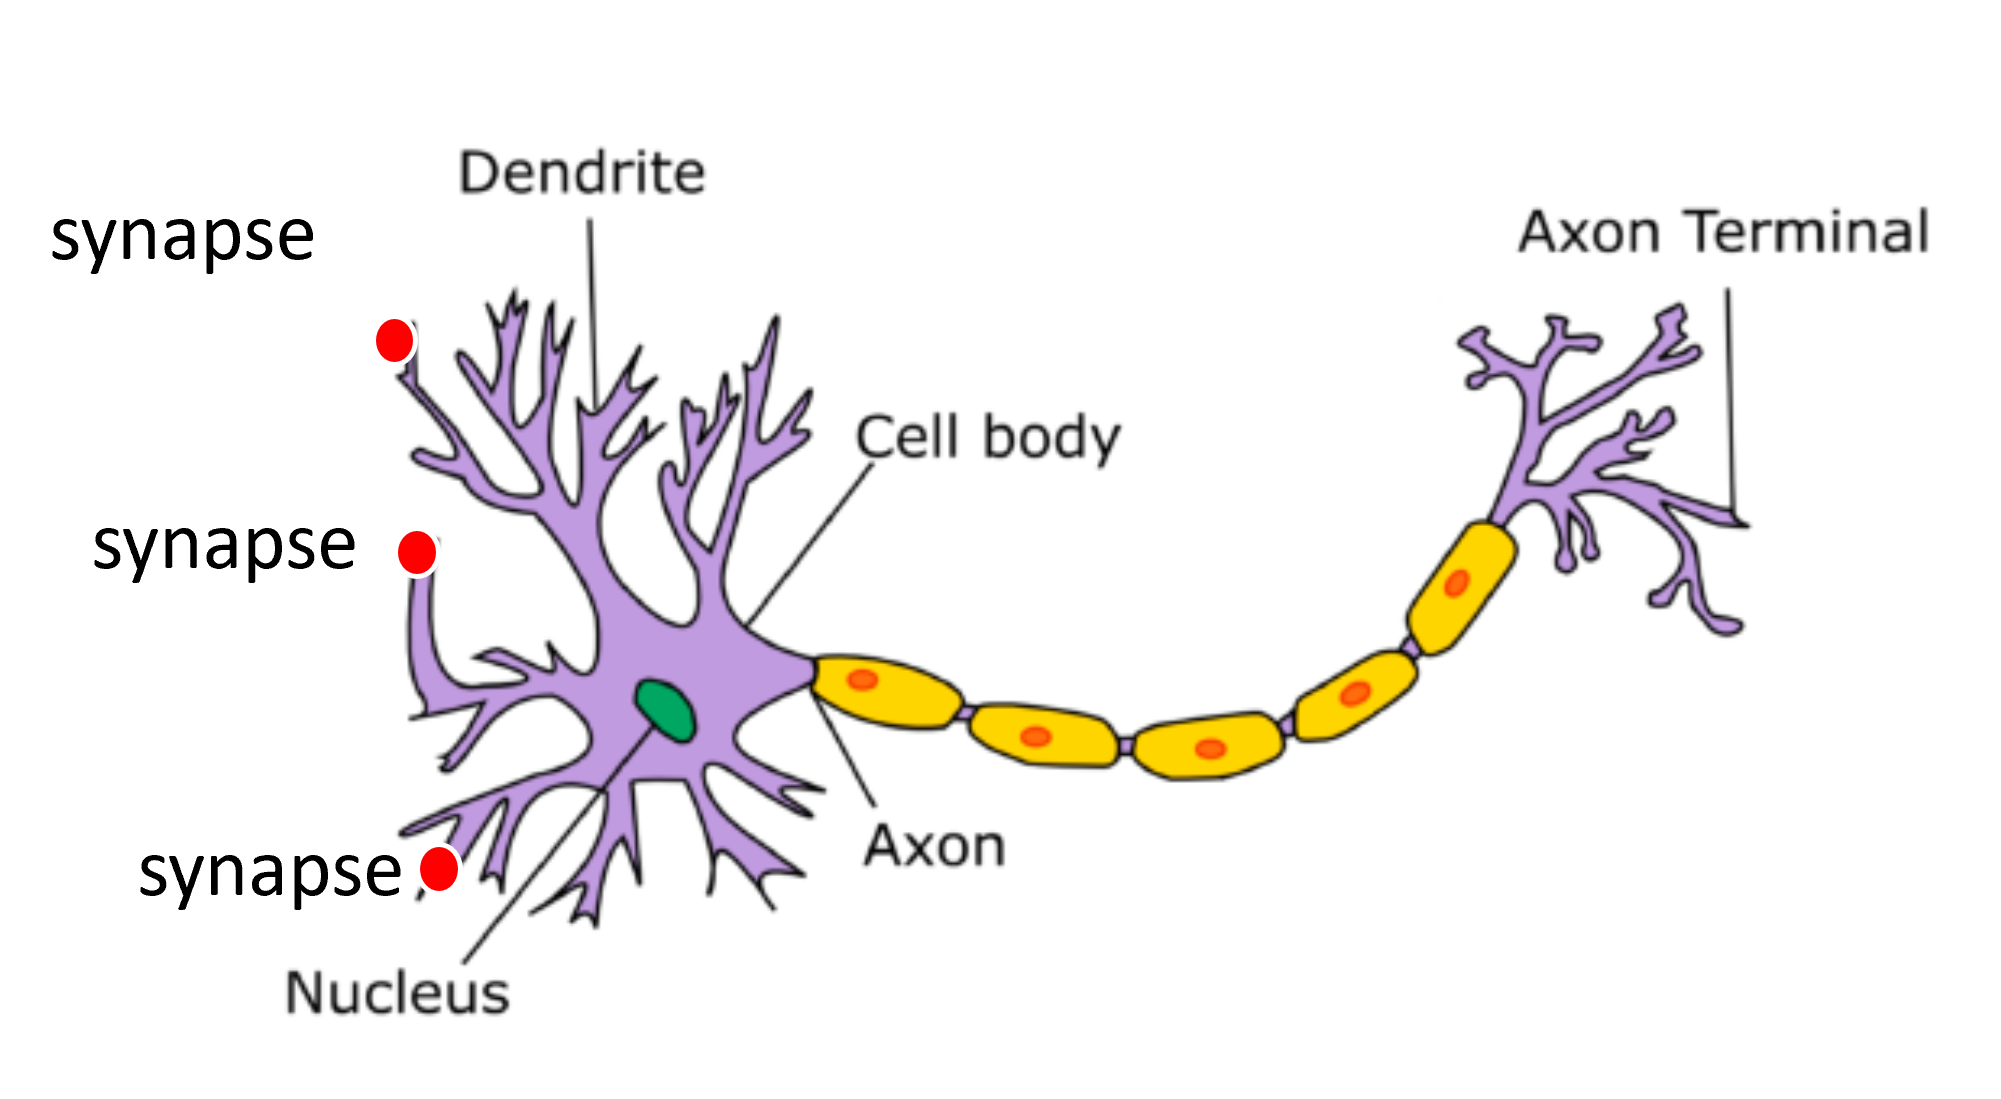
\includegraphics[width=0.75\textwidth]{Topic05fig01.png}
    \caption{Anatomy of a neural cell.}
  \end{figure}
\end{frame}

\begin{frame}{Neuron Components}
  \justifying
  \begin{itemize}
    \item \textbf{Synapse:} interface that modifies or \textit{weights} a signal.
    \item \textbf{Dendrites:} structures that bring signals to the cell body.
    \item \textbf{Cell body:} aggregates inputs and activates the aggregated signal.
    \item \textbf{Axons:} carry the activated signal to the next neuron.
  \end{itemize}
\end{frame}

\begin{frame}{Input Representation}
  \justifying
  We model a neuron receiving $D$ input values:
  \[
    \bm{x} = [x_1, x_2, \cdots, x_D].
  \]
  Each input is weighted and aggregated to produce a linear signal.
\end{frame}

\begin{frame}{Weighted Summation}
  \justifying
  The neuron body aggregates weighted inputs and a bias term:
  \[
    u(\bm{x}) = \sum_{i=1}^{D} w_i x_i + b.
  \]
  This defines a linear hyperplane function in the input space.
\end{frame}

\begin{frame}{Activation and Output}
  \justifying
  \begin{conceptbox}{Perceptron Model}
    \[
      y = f\bigl(u(\bm{x})\bigr) = f\Bigl(\langle \bm{w}, \bm{x} \rangle + b\Bigr).
    \]
  \end{conceptbox}
  The activation function $f(\cdot)$ introduces nonlinearity in the response.
\end{frame}

\begin{frame}{Perceptron as ANN Unit}
  \justifying
  The perceptron is the simplest artificial neural network model.
  In modern usage, a perceptron is a building block used in multi-layer networks.
\end{frame}

\begin{frame}{Perceptron Diagram}
  \justifying
  \begin{figure}[ht]
    \centering
    \begin{subfigure}[b]{0.5\textwidth}
      \centering
      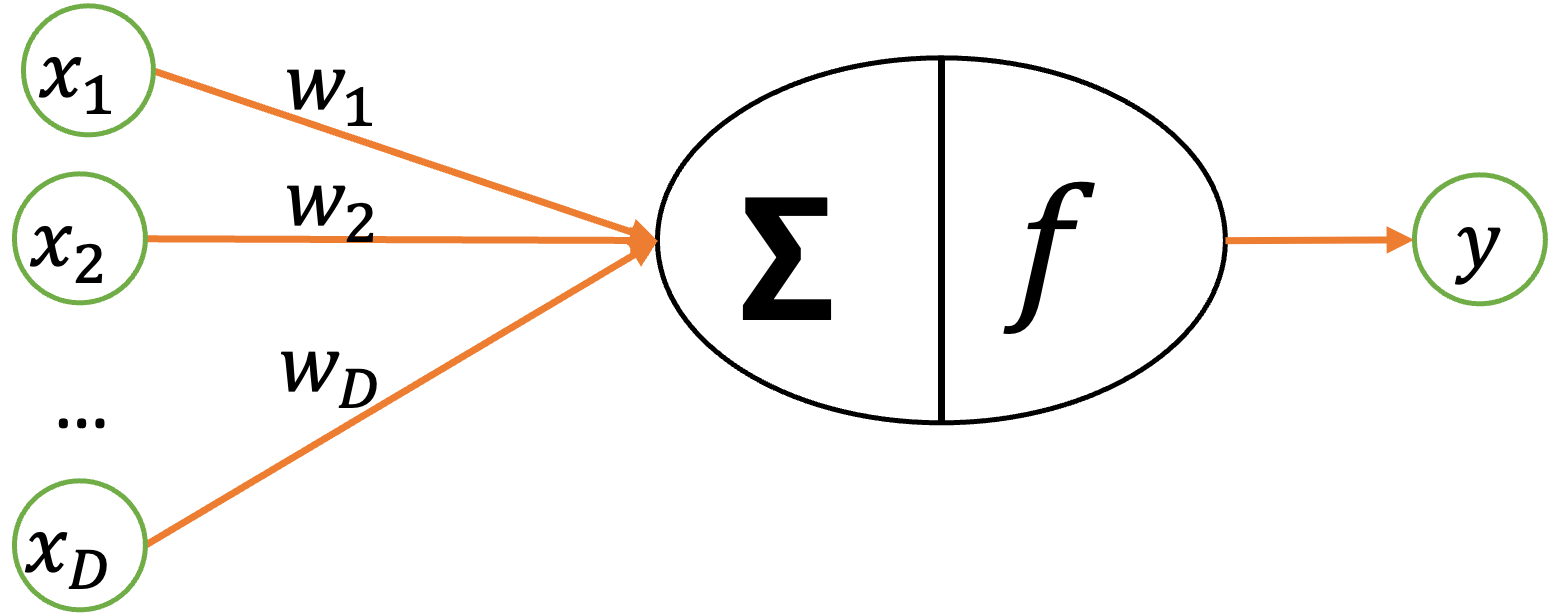
\includegraphics[width=1\textwidth]{Topic05fig02.png}
      \caption{}
    \end{subfigure}
    \begin{subfigure}[b]{0.5\textwidth}
      \centering
      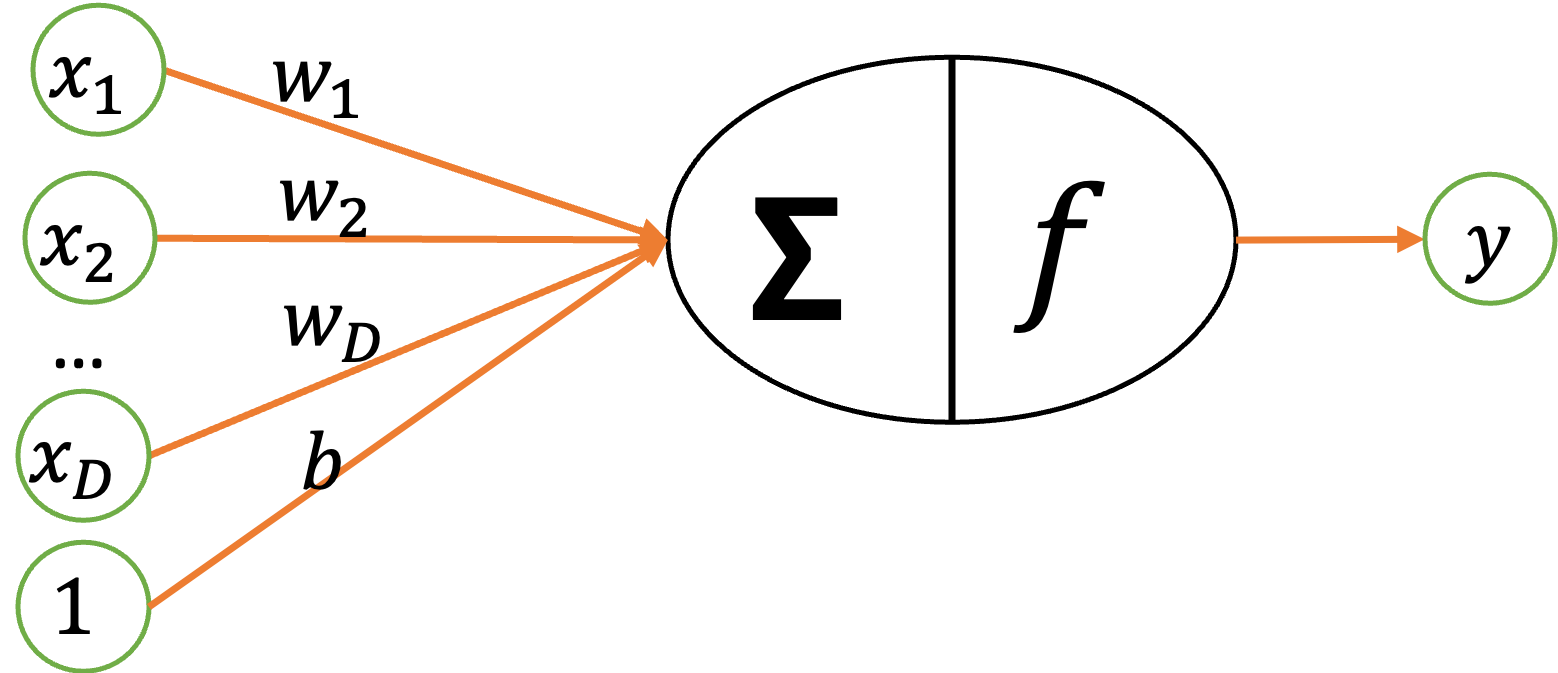
\includegraphics[width=1\textwidth]{Topic05fig03.png}
      \caption{}
    \end{subfigure}
    \caption{Modeling a single neuron: intercept in the body vs. unit input for bias.}
  \end{figure}
\end{frame}

\begin{frame}{Bias as a Weight}
  \justifying
  Treat the bias as a weight by appending a unit input:
  \[
    y = f\Bigl(\sum_{i=1}^{D} w_i x_i + b \cdot 1\Bigr)
      = f\Bigl(\langle \bm{w}', \bm{x}' \rangle\Bigr).
  \]
  \[\bm{w}' = [w_1, \ldots, w_D, b], \quad \bm{x}' = [x_1, \ldots, x_D, 1].\]
\end{frame}

\begin{frame}{Compact Notation}
  \justifying
  We often write the perceptron as:
  \[
    y = f\bigl(\langle \bm{w}, \bm{x} \rangle\bigr)
    \quad \text{or} \quad
    y = f\left(\sum_i w_i x_i\right).
  \]
If we express $u(\bm{x}) = \langle \bm{w}, \bm{x} \rangle$, then
\[
  y = f\bigl(u(\bm{x}) \bigr)
  \]
  This is identiical to the discriminative model as we used in the Logistic regression model - \textit{just that $f(\cdot)$ is not necessariliy a sigmoid function. }
\end{frame}

\section{Perceptron as a Classifier}

\begin{frame}{Decision Boundary}
  \justifying
  The equation $u(\bm{x})=0$ defines a linear decision boundary.
  Once $\bm{w}$ is known, the boundary separates two classes.
\end{frame}

\begin{frame}{Hard Activation Functions}
  \justifying
  \begin{itemize}
    \item \textbf{Heaviside step:}
      \[
        f_h(u) = \begin{cases} 1 & u \ge 0, \\ 0 & u < 0. \end{cases}
      \]
    \item \textbf{Sign:}
      \[
        f_s(u) = \begin{cases} 1 & u \ge 0, \\ -1 & u < 0. \end{cases}
      \]
  \end{itemize}
\end{frame}

\begin{frame}{Hard vs. Soft Activations}
  \justifying
  \begin{warningbox}{Differentiability Matters}
    Hard-activation functions are not differentiable, which limits gradient-based optimization.
  \end{warningbox}
  Soft activations (e.g., sigmoid) are continuous and differentiable, enabling gradient descent.
\end{frame}

\begin{frame}{Sigmoid Activation}
  \justifying
  \[
    f(u) = \frac{1}{1 + \exp(-u)}.
  \]
  This maps input to $(0,1)$ and is commonly used for binary classification outputs.

  In this case, the perceptron leads to a Logistic regression model. 
  \vspace{0.5em}
  \footnotesize
  Source: \href{https://cs231n.stanford.edu/slides/2024/lecture_6_part_2.pdf}{cs231n.stanford.edu/...}
\end{frame}

\begin{frame}{Tanh Activation (hyperbolic tangent)}
  \justifying
  \[
    f(u) = \tanh(u) = \frac{e^u - e^{-u}}{e^u + e^{-u}}.
  \]
  The output range is $(-1,1)$, often preferred for hidden layers.
  \vspace{0.5em}
  \footnotesize
  Source: \href{http://deeplearning.stanford.edu/tutorial/supervised/MultiLayerNeuralNetworks/}{deeplearning.stanford.edu/...}
\end{frame}

\begin{frame}{ReLU Activation}
  \justifying
  \[
    \mathrm{ReLU}(u)=
    \begin{cases}
      0, & u < 0,\\
      u, & u \ge 0.
    \end{cases}
  \]
  ReLU is computationally simple and helps mitigate vanishing gradients.
  \vspace{0.5em}
  \footnotesize
  Source: \href{http://deeplearning.stanford.edu/tutorial/supervised/MultiLayerNeuralNetworks/}{deeplearning.stanford.edu/...}
\end{frame}

\begin{frame}{Leaky ReLU and ELU}
  \justifying
  \begin{itemize}
    \item \textbf{Leaky ReLU:} $f(u) = \max(\alpha u, u)$ adds a small slope for $u<0$.
    \item \textbf{ELU:} smooth negative region for faster convergence in practice.
  \end{itemize}
  These variants reduce the risk of dying neurons.
\end{frame}

\begin{frame}{Activation Function Summary}
  \justifying
  \begin{table}[ht]
    \centering
    \begin{tabular}{l l}
      \toprule
      \textbf{Function} & \textbf{Range / Notes} \\
      \midrule
      Sigmoid & $(0,1)$, saturating, probabilistic output \\
      Tanh & $(-1,1)$, zero-centered \\
      ReLU & $[0,\infty)$, sparse, non-saturating for $u>0$ \\
      Leaky ReLU & Avoids zero gradient for $u<0$ \\
      ELU & Smooth negative side \\
      \bottomrule
    \end{tabular}
  \end{table}
\end{frame}

\begin{frame}{Activation Effects on Optimization}
  \justifying
  \begin{itemize}
    \item Saturating activations (sigmoid, tanh) can cause vanishing gradients.
    \item ReLU can lead to \textit{dying} neurons if many inputs are negative.
    \item Activation choice affects convergence speed and final accuracy.
  \end{itemize}
\end{frame}

\section{Perceptron Learning}

\begin{frame}{Training Data}
  \justifying
  Assume a labeled dataset:
  \[
    \mathcal{D} = \{(\bm{x}_i, y_i) \mid i=1,\ldots,N\}, \quad y_i \in \{-1,1\}.
  \]
  The goal is to estimate $\bm{w}$ from data.
\end{frame}

\begin{frame}{Loss with Hard Activation}
  \justifying
  For sign activation:
  \[
    l_i = \left| f_H\bigl(\langle \bm{w}, \bm{x}_i \rangle\bigr) - y_i^* \right|.
  \]
  The loss is $0$ for correct predictions and $2$ for incorrect predictions.
\end{frame}

\begin{frame}{Loss with Soft Activation}
  \justifying
  For differentiable activations:
  \[
    l_i = \left| f\bigl(\langle \bm{w}, \bm{x}_i \rangle\bigr) - y_i^* \right|.
  \]
  Note that herein the predictions are continuous, enabling gradient-based updates. Yet, the loss - which is the L-1 loss or `absolute-differencing' is not differentiable due to the absolute operation. 
  \[
    l_{2i}= || f\bigl(\langle \bm{w}, \bm{x}_i \rangle\bigr) - y_i^* ||^2.
  \]
  In reality, we often square the prediction error, which yields a smooth objective (L2 loss) that is easier to optimize with gradient-based methods
\end{frame}

\begin{frame}{Total Loss and Optimization}
  \justifying
  \begin{itemize}
\item If using L-1 loss
  \[
    L(\bm{w}) = \sum_{i=1}^{N} \left| f\bigl(\langle \bm{w}, \bm{x}_i \rangle\bigr) - y_i^* \right|.
  \]
\item If using L-2 loss
  \[
    L_2(\bm{w}) = \sum_{i=1}^{N} \left( f\bigl(\langle \bm{w}, \bm{x}_i \rangle\bigr) - y_i^* \right)^2.
  \]
\end{itemize}
Then the model is learned or the model parametrers $\bm{w}$ is learned through
  \[
    \bm{w}^* = \arg\min_{\bm{w}} L(\bm{w}).
  \]
\end{frame}

\begin{frame}{Convexity Note}
  \justifying
  \begin{warningbox}{Optimization Caution}
    Logistic regression yields a convex problem, but the perceptron objective is not necessarily convex.
  \end{warningbox}
\end{frame}

\section{Solution and Limitations}

\begin{frame}{Perceptron Algorithm}
  \justifying
  The perceptron algorithm iteratively updates weights using misclassified examples.
  It does not compute a full gradient over the entire dataset each step.
\end{frame}

\begin{frame}{Separable Data}
  \justifying
  \begin{conceptbox}{Convergence Result}
    If the training data are linearly separable and a hard activation is used, the algorithm converges to a separating hyperplane.
  \end{conceptbox}
  Multiple global solutions can exist when separability holds.
\end{frame}

\begin{frame}{Perceptron as Logic Gate}
  \justifying
  A single perceptron can implement logical operators such as AND, OR, and NOR.
  This works only when the data are linearly separable.
\end{frame}

\begin{frame}{Separable vs. Non-Separable}
  \justifying
  \begin{figure}[ht]
    \centering
    \begin{subfigure}[b]{0.45\textwidth}
      \centering
      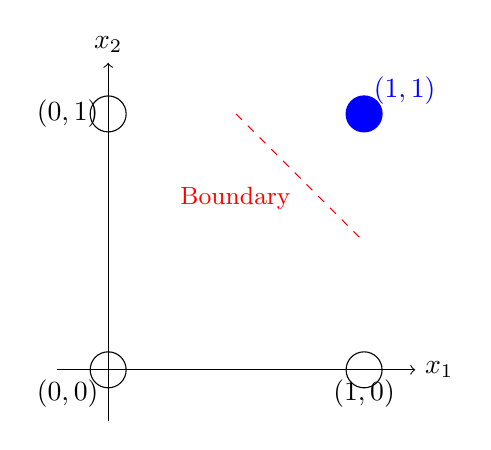
\begin{tikzpicture}[scale=3.25]
        \draw[->] (-0.2,0) -- (1.2,0) node[right]{$x_1$};
        \draw[->] (0,-0.2) -- (0,1.2) node[above]{$x_2$};
        \draw (0,0) circle (2pt) node[below left] {$(0,0)$};
        \draw (0,1) circle (2pt) node[left] {$(0,1)$};
        \draw (1,0) circle (2pt) node[below] {$(1,0)$};
        \filldraw[blue] (1,1) circle (2pt) node[above right] {$(1,1)$};
        \draw[dashed, red] (0.5,1) -- (1,0.5) node[midway, below left] {\small Boundary};
      \end{tikzpicture}
      \caption{Linearly separable (AND).}
    \end{subfigure}
    \hfill
    \begin{subfigure}[b]{0.45\textwidth}
      \centering
      \begin{tikzpicture}[scale=1.25]
        \draw[->] (-0.5,0) -- (3,0) node[right]{$x_1$};
        \draw[->] (0,-0.5) -- (0,3) node[above]{$x_2$};
        \filldraw[blue] (0.5,0.5) circle (3pt) node[below left] {+$\,$};
        \filldraw[blue] (2.5,2.5) circle (3pt) node[above right] {+$\,$};
        \draw (0.5,2.5) circle (3pt) node[above left] {$-\,$};
        \draw (2.5,0.5) circle (3pt) node[below right] {$-\,$};
      \end{tikzpicture}
      \caption{Non-separable (XOR).}
    \end{subfigure}
    \caption{Examples of data configurations in $x_1$-$x_2$ space.}
  \end{figure}
\end{frame}

\begin{frame}{XOR Limitation}
  \justifying
  A single linear decision boundary cannot separate XOR data.
  The minimum loss is nonzero for non-separable configurations.
\end{frame}

\begin{frame}{Why Hidden Layers?}
  \justifying
  \begin{conceptbox}{Key Limitation}
    The decision function $u(\bm{x}) = \langle \bm{w}, \bm{x} \rangle$ is linear.
    Nonlinear boundaries require stacking multiple perceptrons.
  \end{conceptbox}
\end{frame}

\begin{frame}{Bridge to MLP}
  \justifying
  To enhance capacity, we stack multiple perceptrons to form a multi-layer perceptron (MLP).
  The next part introduces MLP architecture and backpropagation.
\end{frame}

\begin{frame}{Part 1 Summary}
  \justifying
  \begin{itemize}
    \item A perceptron computes a weighted sum followed by a nonlinear activation.
    \item Activation choice affects optimization and model behavior.
    \item Linear decision boundaries fail on non-separable data (e.g., XOR).
    \item Multi-layer networks address representational limits.
  \end{itemize}
\end{frame}

\end{document}
